\documentclass{beamer}

%Packages BEGIN
\usepackage{amsmath}
\usepackage{xeCJK} % use this package to set Chinese and English font separately
\usepackage{fontspec} 
\usepackage{hyperref}

%Packages END

%Style setting BEGIN
\usetheme{Madrid} 
\usecolortheme{default} 

% Serif font in Ubuntu. Choose the Chinese font available in your device
\setCJKmainfont{Noto Serif CJK TC}

% Serif font in Ubuntu. Choose the Chinese font available in your device
\setCJKmonofont{Noto Serif CJK TC}

% Serif font in Ubuntu. Choose the Chinese font available in your device
\setCJKsansfont{Noto Serif CJK TC}

\XeTeXlinebreaklocale "zh" % enabling auto linebreaks
\XeTeXlinebreakskip = 0pt plus 1pt % enabling auto linebreaks
 
%Style setting END

\title{Anki Auto-lookup}
\subtitle{A convenient tool for English learning}
\author[張家翔, 王昊謙, 徐鼎翔]
{B08901062 張家翔\inst{1} \and 
B07202020 王昊謙\inst{2} \and 
B07202037 徐鼎翔 \inst{2}}
 
\institute[NTU] % (optional)
{
	\inst{1}%
	Department of Electrical Engineering\\
	National Taiwan University
	\and
	\inst{2}%
	Department of Physics\\
	National Taiwan University
} 

\begin{document}

\frame{\titlepage} 

\begin{frame}{Table of Contents}
	\tableofcontents
\end{frame}

\section{Introduction}%

\begin{frame}{Introduction}
	\begin{itemize}
		\item Anki: a cross-platform flashcard application with API and HTML support.
		\item Goal: a learning tool to help user generate flashcards.
			\begin{itemize}
				\item Automatic lookup
				\item Detailed dictionary entries
				\item Convenient UI
				\item Article analysis
				\item $^*$Image recognition
			\end{itemize}
	\end{itemize}
	Github repository: \url{https://github.com/fhcwcsy/anki-autolookup} 
\end{frame}
\section{Demonstration}%



\section{Detailed Explanation}%

\subsection{Wordlist window}%

\begin{frame}{Wordlist Window}
	\begin{itemize}
		\item \textbf{treading}: multitasking
		\item Inherit from tk.Frame
		\item Adding scrollbar, checkbutton, automatic updates, etc.
	\end{itemize}
\end{frame}

\subsection{Crawler}%

\begin{frame}{Crawler}
	\begin{figure}[h]
		\centering
		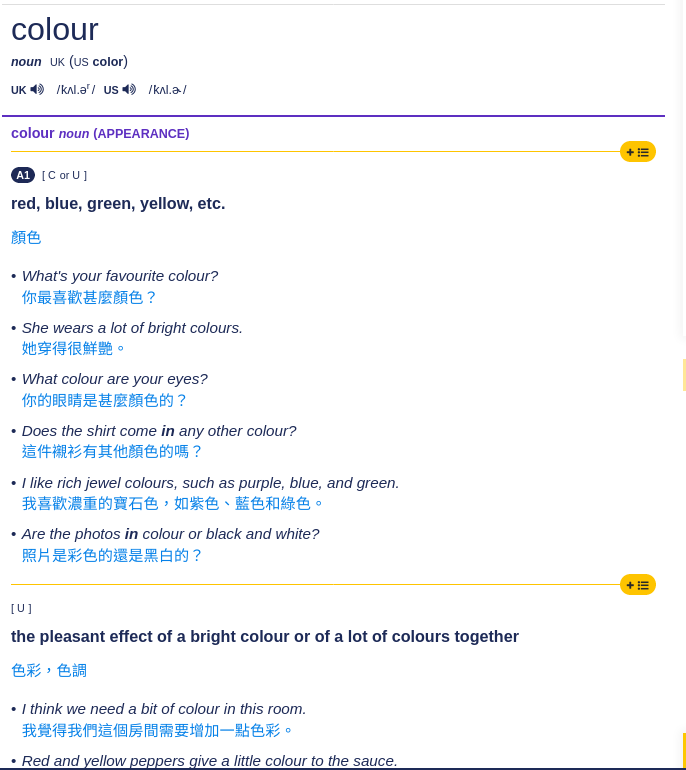
\includegraphics[width=0.6\linewidth]{./cambridge.png}
	\end{figure}
\end{frame}


\subsection{Adding cards}%

\begin{frame}{Adding Cards}
	\textbf{Step 1}: Connect with Anki API.\\
	\textbf{Step 2}: Create a model that contains the fields we need.
	\begin{figure}[h]
			\centering
			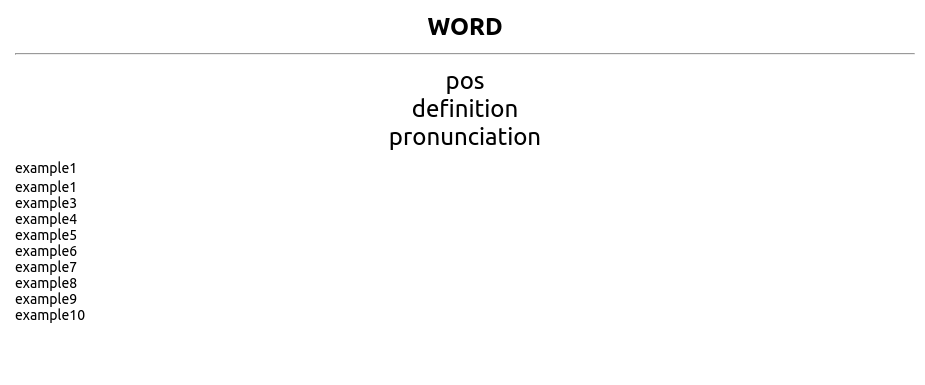
\includegraphics[width=1.00\linewidth]{./model_example.png}
	\end{figure}
\end{frame}

\begin{frame}{Adding Cards}
	\textbf{Step 3}: Create a new card using the information got by the crawler.
	\begin{figure}[h]
			\centering
			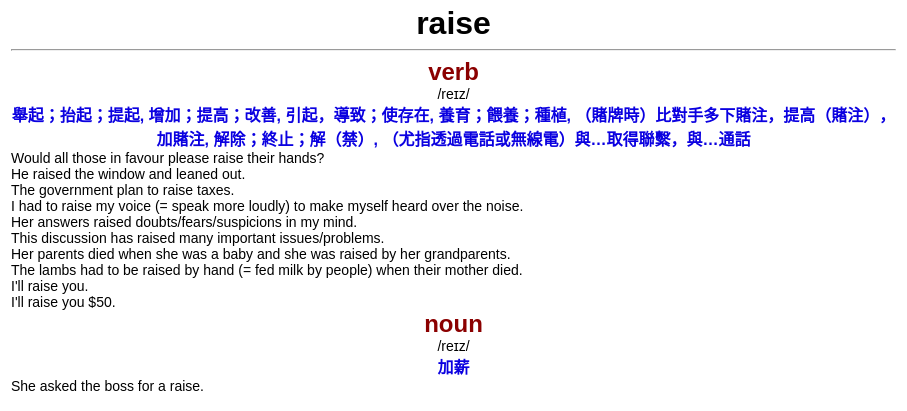
\includegraphics[width=1.0\linewidth]{./card_sample.png}
	\end{figure}
\end{frame}

\subsection{Article analysis}%

\begin{frame}{Article Analysis}
	\begin{itemize}
		\item A dictionary with frequency of english word used in American movie
			subtitles, lyrics, TV shows, etc.
		\item Define vocabulary difficulties as frequency of usage.
	\end{itemize}
\end{frame}

\subsection{GUI}%

\begin{frame}{GUI}
		Module: \textbf{tkinter}\\
		\begin{itemize}
			\item Menu (select decks, select functions)\\
			\begin{itemize}
				\item Word Lookup\\
				\item Article Lookup\\
				\item Image Lookup\\
			\end{itemize}
		\end{itemize}
		\begin{figure}[h]
				\centering
				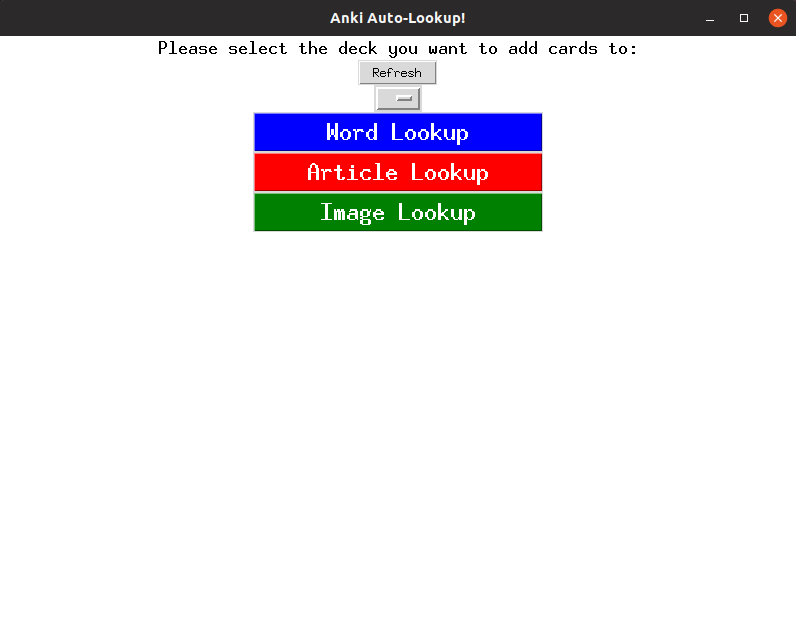
\includegraphics[width=0.6\linewidth]{./GUI_main.png}
		\end{figure}
\end{frame}

\begin{frame}{Word Lookup}
	\begin{enumerate}
		\item When you key in 'Enter', add the line into 'Words to be added' column.
		\item When you press 'Done', add the words into Anki.
	\end{enumerate}
	\begin{figure}[h]
			\centering
			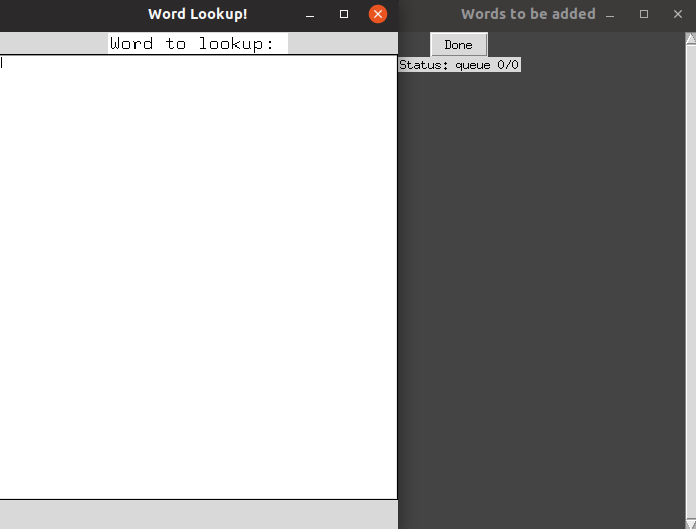
\includegraphics[width=0.6\linewidth]{./word_lookup_gui.png}
	\end{figure}
\end{frame}

\subsection{Image Recognition}%
\label{sub:image_recognition}



\begin{frame}
	\frametitle{Image Recognization}
	\textbf{Goal}: Indentify words in a picture and generate flashcards.
	\begin{figure}[h]
		\centering
		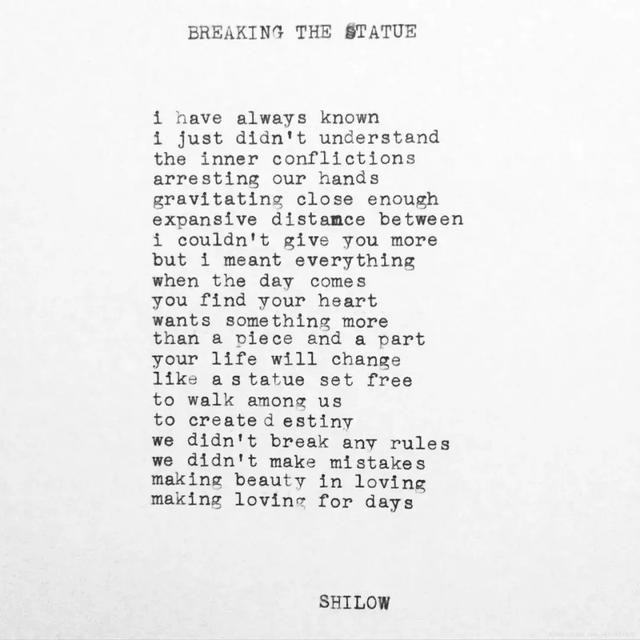
\includegraphics[width=0.55\linewidth]{./img1.jpg}
		\caption{Target picture}
	\end{figure}
\end{frame}

\begin{frame}{Method}
		\textbf{Step 1}: Convert the picture to grayscale, then set the darker pixels to absolute black, lighter pixels to absolute white.\\
		\textbf{Step 1-1}: To implement Step 1, we turn the picture into np.arrays.
		%\begin{figure}[h]
			%\centering
			%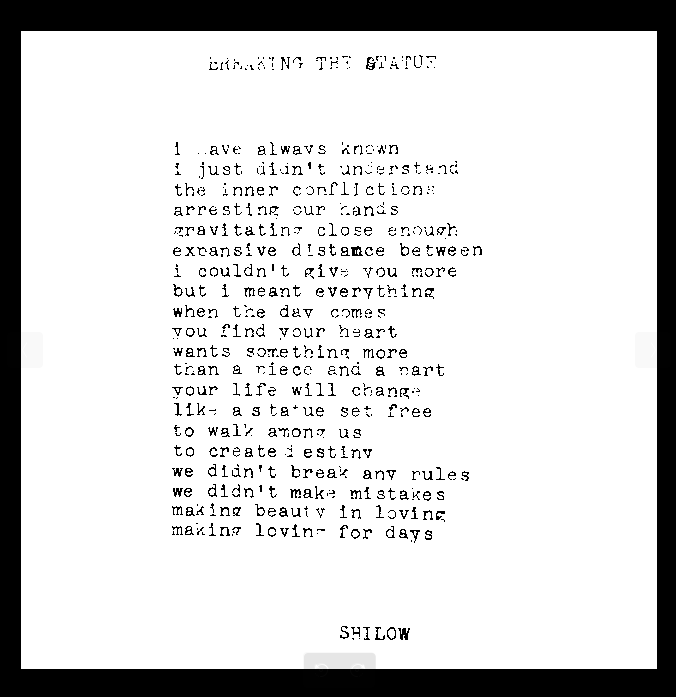
\includegraphics[width=0.50\linewidth]{./picture_blackwhite.png}
		%\end{figure}
\end{frame}

\begin{frame}{Task}
		\textbf{How do computers recognize a word?}
		\begin{figure}[h]
			\centering
			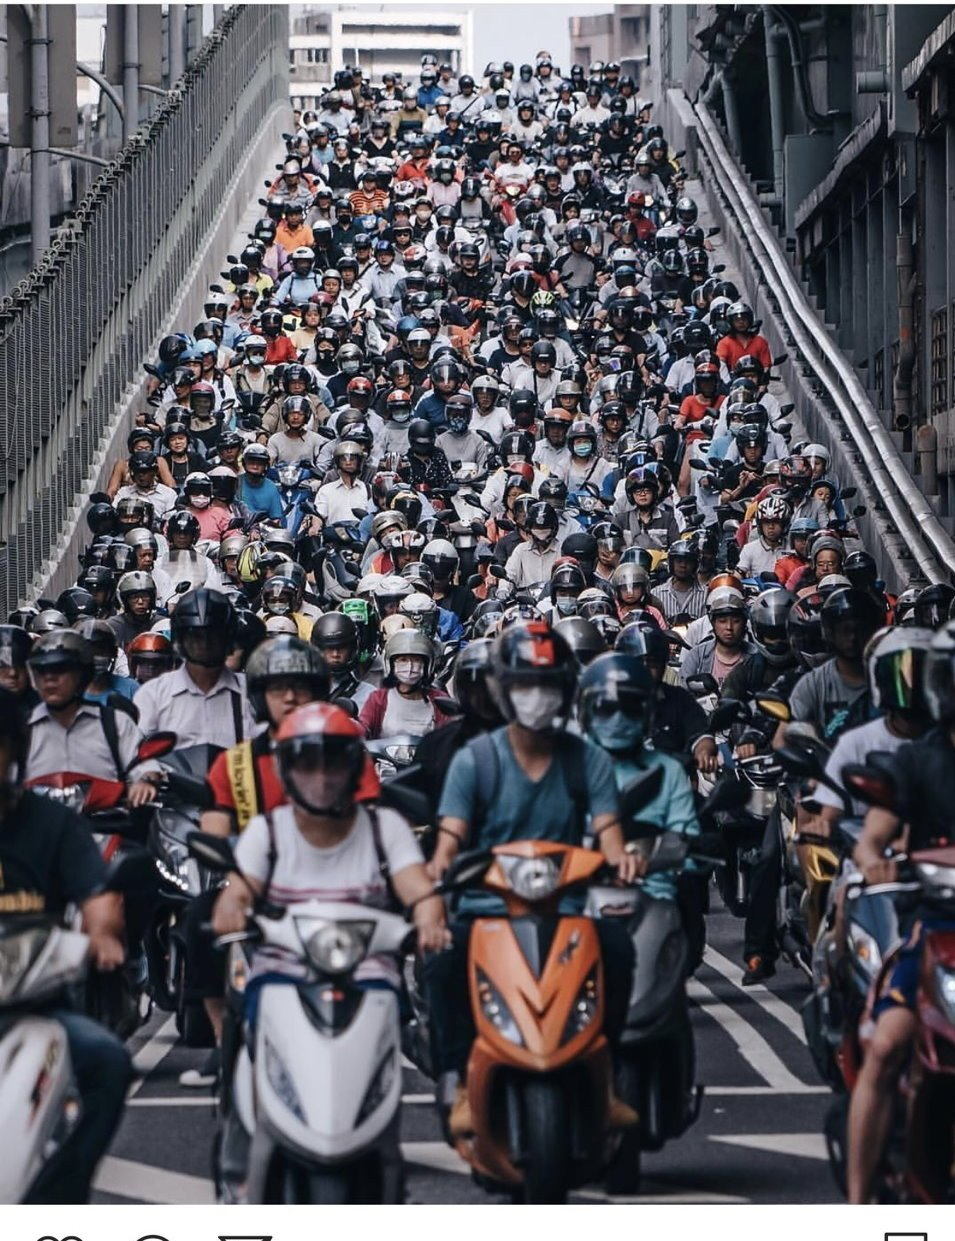
\includegraphics[width=0.55\linewidth]{./motor.jpg}
		\end{figure}
\end{frame}

\begin{frame}{Fourier Transform}
	\textbf{Seems good...but does it?}
		\begin{figure}[H]
			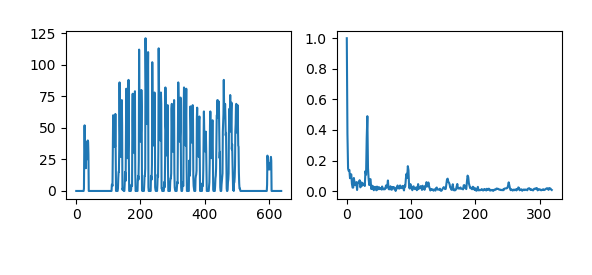
\includegraphics[width=0.45\linewidth]{./fourier.png}
			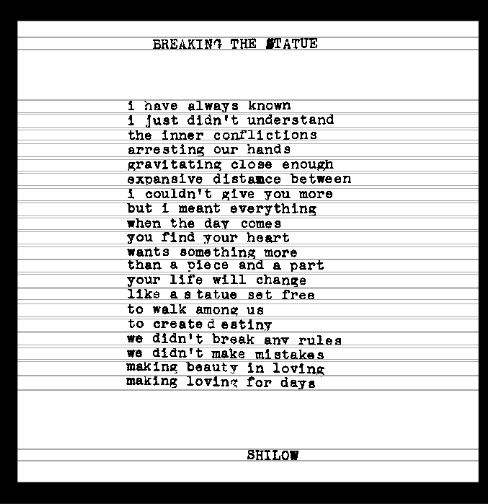
\includegraphics[width=0.55\linewidth]{./imgslice.png}
		\end{figure}
\end{frame}

\begin{frame}{Fourier Transform}
	\textbf{Fewer data lead to less precision.}
	\begin{figure}[H]
		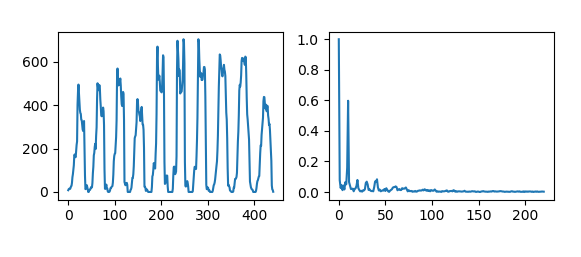
\includegraphics[width=0.55\linewidth]{./fourier2.png}
		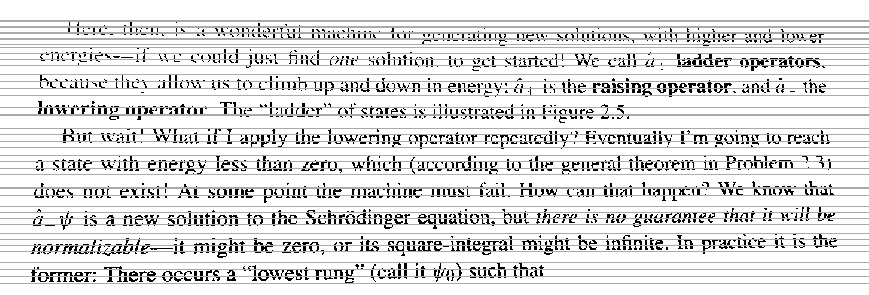
\includegraphics[width=0.70\linewidth]{./imgslice2.png}
	\end{figure}
\end{frame}

\begin{frame}{Method}
	\textbf{Step 2-1}: When the number of black pixels on a row (of pixels) is below a threshold, the row is recognized as the boundary of the line.\\
		\textbf{Step 2-2}: Detect the wider white columns to identify words.\\
		\begin{figure}[h]
			\centering
			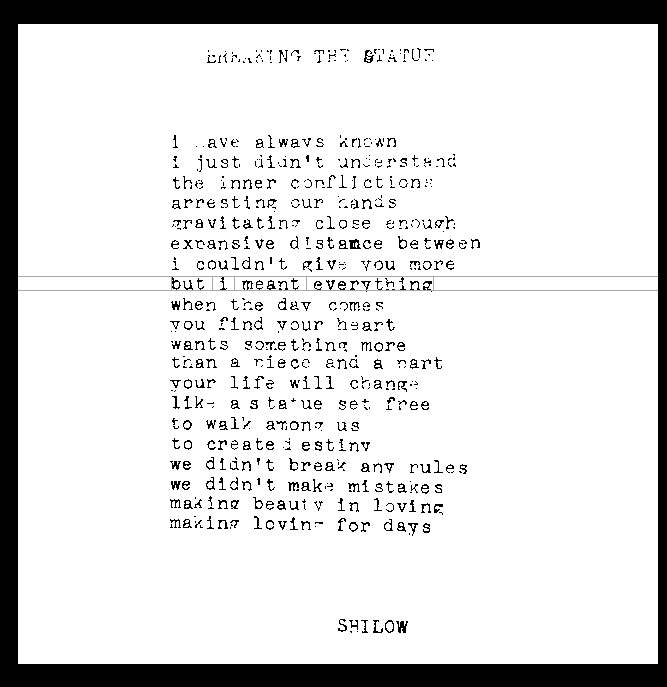
\includegraphics[width=0.50\linewidth]{./raw_done.png}
		\end{figure}
\end{frame}

\begin{frame}{Method}
		\textbf{Step 3-1}: Detect the words in the line, use the order to determine which word I selected. We get WordFromLine.\\
		\textbf{Step 3-2}: Detect the word in the region I selected. We get WordFromWord.\\
		\textbf{Step 3-3}: If the WordFromLine is similar to WordFromWord or len(WordFromWord)=0, return WordFromLine. Else, return WordFromWord.\\
		\begin{figure}[h]
			\centering
			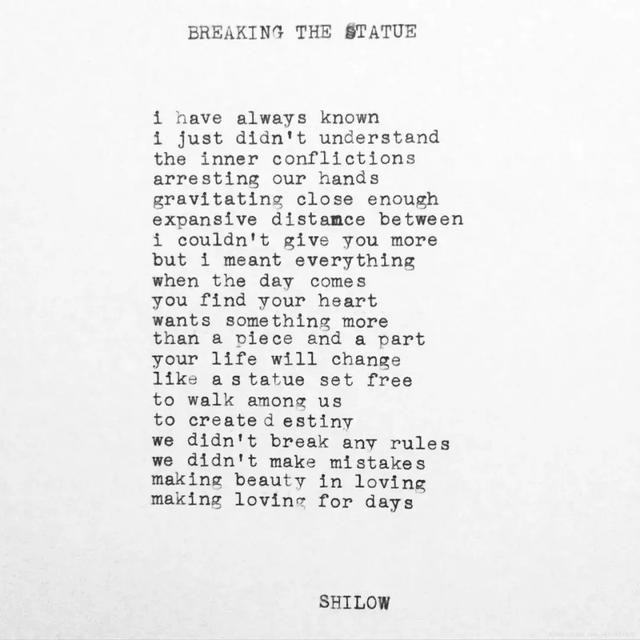
\includegraphics[height=0.4\linewidth]{./img1.jpg}
			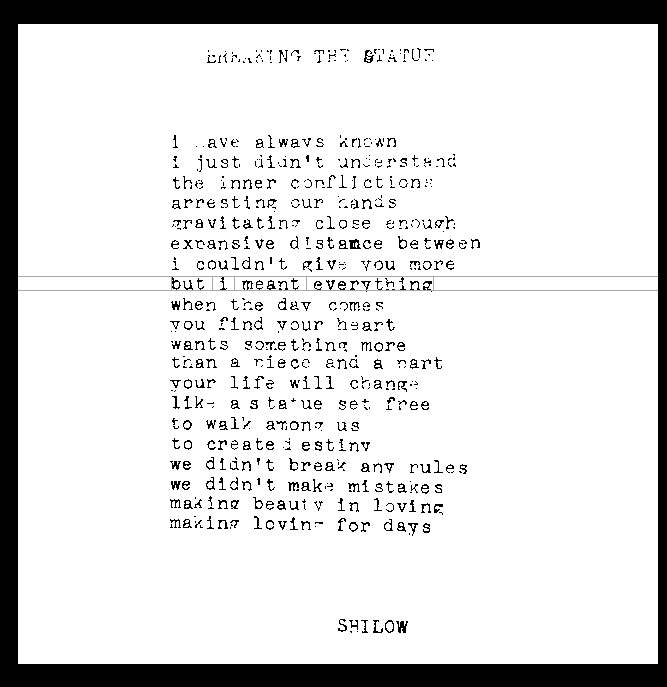
\includegraphics[width = 0.4\linewidth]{./raw_done.png}
		\end{figure}
\end{frame}
 



\end{document}
